\documentclass[a4paper, 12pt]{article}
\topmargin-2.0cm

\usepackage{graphicx}
\usepackage{subfig}
\usepackage{listings}
\usepackage{color}
\usepackage{fancyvrb}
\usepackage[usenames,dvipsnames]{xcolor}


\advance\oddsidemargin-0.65in
%\textheight 9.25in
\textheight 10in
\textwidth 6.75in
\newcommand\bb[1]{\mbox{\em #1}}
\def\baselinestretch{1.05}

\newcommand{\hsp}{\hspace*{\parindent}}

%\usepackage[english,frenchb]{babel} %---- frenchb for french option of babel == francais (otherwise if "french", babel tries to load french 					     % package from B.Gaulle)
%\usepackage{ucs}
%\usepackage[utf8x]{inputenc} %--- for UTF8 encoding
%\usepackage[latin1]{inputenc} %--- for iso-8859-1 encoding 
%--- conversion en ligne de l'encodage 
% iconv -f utf8 -t iso8859-1 fichieroriginal -o fichiertransformé
%
%\usepackage[T1]{fontenc}



\fvset{frame=single,framesep=1mm,fontfamily=courier,fontsize=\scriptsize,framerule=.3mm,numbersep=1mm,commandchars=\\\{\}}


\begin{document}

\renewcommand{\contentsname}{}


\vspace*{1cm}
\begin{center}
{\LARGE \bf Firmware updates -- May 2015 -- v0.3}\\
\vspace*{0.1cm}
%{\normalsize Jean-Baptiste Sauvan (sauvan@llr.in2p3.fr)}
\end{center}
\vspace*{1cm}


\begin{figure}[hbtp]
  \begin{center}
    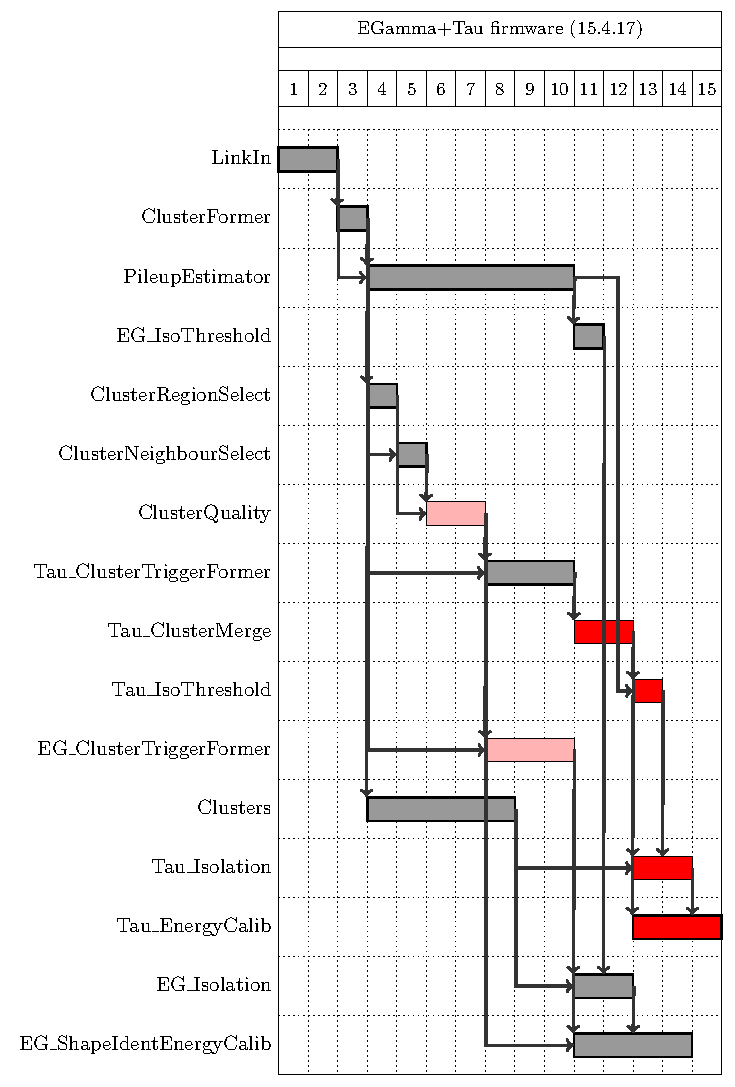
\includegraphics[width=11cm]{./gantt_charts/firmware_egAndTau_mod.pdf}
    \caption{Timing and relation graph of the EGamma and Tau firmware. Each row corresponds to a given module of the algorithm, while the columns indicate the clock number. Gray modules are modules that don't require updates with respect to the current firmware implementation. Pink modules require updates or fixes. Red modules are currently not existing.}
    \label{fig:gantt}
  \end{center}
\end{figure}

\newpage

In the following, the updates to the current EGamma firmware are listed. Modifications of existing code are detailed in a pseudo-code form. Code to be removed is indicated in red, while code to be added is indicated in blue; black code doesn't need changes.
%
\section{Reduction of the number of instances}
The modifications related to the reduction of the number of potential candidates from $72$ to $36$ in each slice are not detailed here. It is just mentioned that this reduction can be done right after the seed filtering (section~\ref{sec:filter} below) and before the sharing (section~\ref{sec:sharing1}).


\section{ClusterQuality}
\subsection{ClusterThresholdQuality}
The only update here is the corner trimming that should be removed. 

\begin{Verbatim}[label={Trimming updates}]
\textcolor{red}{if(R1N<clusterThreshold and R1E<clusterThreshold) keepTower_R1NE=false}
\textcolor{red}{if(R1S<clusterThreshold and R1E<clusterThreshold) keepTower_R1SE=false}
\textcolor{red}{if(R1N<clusterThreshold and R1W<clusterThreshold) keepTower_R1NW=false}
\textcolor{red}{if(R1S<clusterThreshold and R1W<clusterThreshold) keepTower_R1SW=false}
\end{Verbatim}

\subsection{EGammaFilteringQuality}\label{sec:filter}
The updates in the filtering correspond to fixes that have been made in the emulator since the egamma algorithm specifications have been written. There are two main fixes:
\begin{itemize}
  \item The conditions for the negative boundary should be the same as for the positive boundary.
  \item When looking at towers in the second ring (R2), clusters should be invalidated only if the tower in-between pass the clustering threshold. 
\end{itemize}
%
There are in addition a few inconsistencies in the current VHDL code. \\
Fixes are listed below.


\begin{Verbatim}[label={Filtering updates}]
\textit{//******************************************************************//}
\textit{// Positive eta}
if(iEta>1) 
  \textcolor{blue}{if(R2N  >  C and R1N >= clusterThreshold) invalidateCluster}
  if(R1N  >  C) invalidateCluster
  if(R1NE >  C) invalidateCluster
  if(R1E  >  C) invalidateCluster
  if(R1SE >  C) invalidateCluster
  if(R1S  >= C) invalidateCluster
  if(R1SW >= C) invalidateCluster
  if(R1W  >= C) invalidateCluster
  if(R1NW >= C) invalidateCluster
  \textcolor{red}{if(R2S  >= C) invalidateCluster}
  \textcolor{blue}{if(R2S  >= C and R1S >= clusterThreshold) invalidateCluster}
\textit{//******************************************************************//}
\textit{// Negative eta}
\textcolor{red}{else if(iEta<0)}
\textcolor{blue}{else if(iEta<-1)}
  \textcolor{red}{if(R2N  >= C) invalidateCluster}
  \textcolor{blue}{if(R2N  >= C and R1N >= clusterThreshold) invalidateCluster}
  if(R1N  >= C) invalidateCluster
  if(R1NE >= C) invalidateCluster
  if(R1E  >= C) invalidateCluster
  if(R1SE >= C) invalidateCluster
  if(R1S  >  C) invalidateCluster
  if(R1SW >  C) invalidateCluster
  if(R1W  >  C) invalidateCluster
  if(R1NW >  C) invalidateCluster
  \textcolor{blue}{if(R2S  >  C and R1S >= clusterThreshold) invalidateCluster}
\textit{//******************************************************************//}
\textit{// Central boundary}
\textcolor{red}{else if(iEta=1)}
\textcolor{blue}{else if(iEta=1 or iEta=-1)}
  \textcolor{blue}{if(R2N  >  C and R1N >= clusterThreshold) invalidateCluster}
  if(R1N  >  C) invalidateCluster
  if(R1NE >  C) invalidateCluster
  if(R1E  >  C) invalidateCluster
  if(R1SE >  C) invalidateCluster
  if(R1S  >= C) invalidateCluster
  if(R1SW >  C) invalidateCluster
  if(R1W  >  C) invalidateCluster
  if(R1NW >  C) invalidateCluster
  \textcolor{red}{if(R2S  >= C) invalidateCluster}
  \textcolor{blue}{if(R2S  >= C and R1S >= clusterThreshold) invalidateCluster}
\textit{//******************************************************************//}
\end{Verbatim}


\subsection{EGammaSharingQuality}\label{sec:sharing1}
The updates in the sharing correspond also to fixes that have been made in the emulator since the egamma algorithm specifications have been written. They are mainly related to the way towers at $i\phi=\pm2$ are shared between two seeds.

\begin{Verbatim}[label={Sharing updates}]
\textit{//******************************************************************//}
\textit{// Positive eta}
if(iEta>1) 
  if R2N > C 
    keepTower_R1NW = false
    keepTower_R1N  = false
    keepTower_R1NE = false
  if R2NNE > C
    keepTower_R1N  = false
    keepTower_R1NE = false
    \textcolor{blue}{keepTower_R2N  = false}
    \textcolor{blue}{if(R1NE >= clusterThreshold) keepTower_R1E = false}
  if R2SSE > C
    keepTower_R1S  = false
    keepTower_R1SE = false
    \textcolor{blue}{keepTower_R2S  = false}
    \textcolor{blue}{if(R1SE >= clusterThreshold) keepTower_R1E = false}
  if R2S >= C
    keepTower_R1SW = false
    keepTower_R1S  = false
    keepTower_R1SE = false
  if R2SSW >= C
    keepTower_R1SW = false
    keepTower_R1S  = false
    \textcolor{blue}{keepTower_R2S  = false}
    \textcolor{blue}{if(R1SW >= clusterThreshold) keepTower_R1W = false}
  if R2NNW >= C
    keepTower_R1NW = false
    keepTower_R1N  = false
    \textcolor{blue}{keepTower_R2N  = false}
    \textcolor{blue}{if(R1NW >= clusterThreshold) keepTower_R1W = false}
  if R3N > C
    \textcolor{red}{keepTower_R1N = false}
    \textcolor{blue}{if(R2N >= clusterThreshold) keepTower_R1N = false}
    keepTower_R2N = false
  if R3NE > C
    \textcolor{red}{keepTower_R1NE = false}
    \textcolor{blue}{if(R2NNE >= clusterThreshold) keepTower_R1NE = false}
    keepTower_R2N  = false
  if R3NW >= C
    \textcolor{red}{keepTower_R1NW = false}
    \textcolor{blue}{if(R2NNW >= clusterThreshold) keepTower_R1NW = false}
    keepTower_R2N  = false
  if R3S >= C
    \textcolor{red}{keepTower_R1S = false}
    \textcolor{blue}{if(R2S >= clusterThreshold) keepTower_R1S = false}
    keepTower_R2S = false
  if R3SE > C
    \textcolor{red}{keepTower_R1SE = false}
    \textcolor{blue}{if(R2SSE >= clusterThreshold) keepTower_R1SE = false}
    keepTower_R2S  = false
  if R3SW >= C
    \textcolor{red}{keepTower_R1SW = false}
    \textcolor{blue}{if(R2SSW >= clusterThreshold) keepTower_R1SW = false}
    keepTower_R2S  = false
  if R4N > C
    \textcolor{red}{keepTower_R1N = false}
    \textcolor{red}{keepTower_R2N = false}
    \textcolor{blue}{if(R3N >= clusterThreshold) keepTower_R2N = false}
  if R4S >= C
    \textcolor{red}{keepTower_R1S = false}
    \textcolor{red}{keepTower_R2S = false}
    \textcolor{blue}{if(R3S >= clusterThreshold) keepTower_R2S = false}
\textit{//******************************************************************//}
\textit{// Boundary Positive eta}
if(iEta=1) 
  if R2N > C 
    keepTower_R1NW = false
    keepTower_R1N  = false
    keepTower_R1NE = false
  if R2NNE > C
    keepTower_R1N  = false
    keepTower_R1NE = false
    \textcolor{blue}{keepTower_R2N  = false}
    \textcolor{blue}{if(R1NE >= clusterThreshold) keepTower_R1E = false}
  if R2SSE > C
    keepTower_R1S  = false
    keepTower_R1SE = false
    \textcolor{blue}{keepTower_R2S  = false}
    \textcolor{blue}{if(R1SE >= clusterThreshold) keepTower_R1E = false}
  if R2S >= C
    keepTower_R1SW = false
    keepTower_R1S  = false
    keepTower_R1SE = false
  if R2SSW >= C
    keepTower_R1SW = false
    keepTower_R1S  = false
    \textcolor{blue}{keepTower_R2S  = false}
    \textcolor{blue}{if(R1SW >= clusterThreshold) keepTower_R1W = false}
  if R2NNW > C
    keepTower_R1NW = false
    keepTower_R1N  = false
    \textcolor{blue}{keepTower_R2N  = false}
    \textcolor{blue}{if(R1NW >= clusterThreshold) keepTower_R1W = false}
  if R3N > C
    \textcolor{red}{keepTower_R1N = false}
    \textcolor{blue}{if(R2N >= clusterThreshold) keepTower_R1N = false}
    keepTower_R2N = false
  if R3NE > C
    \textcolor{red}{keepTower_R1NE = false}
    \textcolor{blue}{if(R2NNE >= clusterThreshold) keepTower_R1NE = false}
    keepTower_R2N  = false
  if R3NW > C
    \textcolor{red}{keepTower_R1NW = false}
    \textcolor{blue}{if(R2NNW >= clusterThreshold) keepTower_R1NW = false}
    keepTower_R2N  = false
  if R3S >= C
    \textcolor{red}{keepTower_R1S = false}
    \textcolor{blue}{if(R2S >= clusterThreshold) keepTower_R1S = false}
    keepTower_R2S = false
  if R3SE > C
    \textcolor{red}{keepTower_R1SE = false}
    \textcolor{blue}{if(R2SSE >= clusterThreshold) keepTower_R1SE = false}
    keepTower_R2S  = false
  if R3SW >= C
    \textcolor{red}{keepTower_R1SW = false}
    \textcolor{blue}{if(R2SSW >= clusterThreshold) keepTower_R1SW = false}
    keepTower_R2S  = false
  if R4N > C
    \textcolor{red}{keepTower_R1N = false}
    \textcolor{red}{keepTower_R2N = false}
    \textcolor{blue}{if(R3N >= clusterThreshold) keepTower_R2N = false}
  if R4S >= C
    \textcolor{red}{keepTower_R1S = false}
    \textcolor{red}{keepTower_R2S = false}
    \textcolor{blue}{if(R3S >= clusterThreshold) keepTower_R2S = false}
\textit{//******************************************************************//}
\textit{// Negative eta}
if(iEta<-1) 
  if R2N >= C 
    keepTower_R1NW = false
    keepTower_R1N  = false
    keepTower_R1NE = false
  if R2NNE >= C
    keepTower_R1N  = false
    keepTower_R1NE = false
    \textcolor{blue}{keepTower_R2N  = false}
    \textcolor{blue}{if(R1NE >= clusterThreshold) keepTower_R1E = false}
  if R2SSE >= C
    keepTower_R1S  = false
    keepTower_R1SE = false
    \textcolor{blue}{keepTower_R2S  = false}
    \textcolor{blue}{if(R1SE >= clusterThreshold) keepTower_R1E = false}
  if R2S > C
    keepTower_R1SW = false
    keepTower_R1S  = false
    keepTower_R1SE = false
  if R2SSW > C
    keepTower_R1SW = false
    keepTower_R1S  = false
    \textcolor{blue}{keepTower_R2S  = false}
    \textcolor{blue}{if(R1SW >= clusterThreshold) keepTower_R1W = false}
  if R2NNW > C
    keepTower_R1NW = false
    keepTower_R1N  = false
    \textcolor{blue}{keepTower_R2N  = false}
    \textcolor{blue}{if(R1NW >= clusterThreshold) keepTower_R1W = false}
  if R3N >= C
    \textcolor{red}{keepTower_R1N = false}
    \textcolor{blue}{if(R2N >= clusterThreshold) keepTower_R1N = false}
    keepTower_R2N = false
  if R3NE >= C
    \textcolor{red}{keepTower_R1NE = false}
    \textcolor{blue}{if(R2NNE >= clusterThreshold) keepTower_R1NE = false}
    keepTower_R2N  = false
  if R3NW > C
    \textcolor{red}{keepTower_R1NW = false}
    \textcolor{blue}{if(R2NNW >= clusterThreshold) keepTower_R1NW = false}
    keepTower_R2N  = false
  if R3S > C
    \textcolor{red}{keepTower_R1S = false}
    \textcolor{blue}{if(R2S >= clusterThreshold) keepTower_R1S = false}
    keepTower_R2S = false
  if R3SE >= C
    \textcolor{red}{keepTower_R1SE = false}
    \textcolor{blue}{if(R2SSE >= clusterThreshold) keepTower_R1SE = false}
    keepTower_R2S  = false
  if R3SW > C
    \textcolor{red}{keepTower_R1SW = false}
    \textcolor{blue}{if(R2SSW >= clusterThreshold) keepTower_R1SW = false}
    keepTower_R2S  = false
  if R4N >= C
    \textcolor{red}{keepTower_R1N = false}
    \textcolor{red}{keepTower_R2N = false}
    \textcolor{blue}{if(R3N >= clusterThreshold) keepTower_R2N = false}
  if R4S > C
    \textcolor{red}{keepTower_R1S = false}
    \textcolor{red}{keepTower_R2S = false}
    \textcolor{blue}{if(R3S >= clusterThreshold) keepTower_R2S = false}
\textit{//******************************************************************//}
\textit{// Boundary Negative eta}
if(iEta=-1) 
  if R2N > C 
    keepTower_R1NW = false
    keepTower_R1N  = false
    keepTower_R1NE = false
  if R2NNE > C
    keepTower_R1N  = false
    keepTower_R1NE = false
    \textcolor{blue}{keepTower_R2N  = false}
    \textcolor{blue}{if(R1NE >= clusterThreshold) keepTower_R1E = false}
  if R2SSE >= C
    keepTower_R1S  = false
    keepTower_R1SE = false
    \textcolor{blue}{keepTower_R2S  = false}
    \textcolor{blue}{if(R1SE >= clusterThreshold) keepTower_R1E = false}
  if R2S >= C
    keepTower_R1SW = false
    keepTower_R1S  = false
    keepTower_R1SE = false
  if R2SSW > C
    keepTower_R1SW = false
    keepTower_R1S  = false
    \textcolor{blue}{keepTower_R2S  = false}
    \textcolor{blue}{if(R1SW >= clusterThreshold) keepTower_R1W = false}
  if R2NNW > C
    keepTower_R1NW = false
    keepTower_R1N  = false
    \textcolor{blue}{keepTower_R2N  = false}
    \textcolor{blue}{if(R1NW >= clusterThreshold) keepTower_R1W = false}
  if R3N > C
    \textcolor{red}{keepTower_R1N = false}
    \textcolor{blue}{if(R2N >= clusterThreshold) keepTower_R1N = false}
    keepTower_R2N = false
  if R3NE > C
    \textcolor{red}{keepTower_R1NE = false}
    \textcolor{blue}{if(R2NNE >= clusterThreshold) keepTower_R1NE = false}
    keepTower_R2N  = false
  if R3NW > C
    \textcolor{red}{keepTower_R1NW = false}
    \textcolor{blue}{if(R2NNW >= clusterThreshold) keepTower_R1NW = false}
    keepTower_R2N  = false
  if R3S >= C
    \textcolor{red}{keepTower_R1S = false}
    \textcolor{blue}{if(R2S >= clusterThreshold) keepTower_R1S = false}
    keepTower_R2S = false
  if R3SE >= C
    \textcolor{red}{keepTower_R1SE = false}
    \textcolor{blue}{if(R2SSE >= clusterThreshold) keepTower_R1SE = false}
    keepTower_R2S  = false
  if R3SW > C
    \textcolor{red}{keepTower_R1SW = false}
    \textcolor{blue}{if(R2SSW >= clusterThreshold) keepTower_R1SW = false}
    keepTower_R2S  = false
  if R4N > C
    \textcolor{red}{keepTower_R1N = false}
    \textcolor{red}{keepTower_R2N = false}
    \textcolor{blue}{if(R3N >= clusterThreshold) keepTower_R2N = false}
  if R4S >= C
    \textcolor{red}{keepTower_R1S = false}
    \textcolor{red}{keepTower_R2S = false}
    \textcolor{blue}{if(R3S >= clusterThreshold) keepTower_R2S = false}
\textit{//******************************************************************//}
\end{Verbatim}

\subsection{EGammaNeighborQuality}
No change.

\section{EGClusterTriggerFormer}
An additional trimming is added on top of the left--right trimming. This additional trimming is specific to egamma clusters. It depends on the cluster flags as well as on the ieta position and is implemented via a LUT (with 12 bits in inputs and 7 bits in output).
%
This additional trimming makes the trigger former module more complicated due to the necessity to compute first the left--right flag before trimming the cluster flags and computing the final cluster energy from the trimmed cluster flags. It should require one more adder as well as more latency from reading the trimming LUT and recomputing partial sums. The updates are detailed below.

\begin{Verbatim}[label={EG cluster energy sums}]
\textit{//******************************************************************//}
\textit{// Tower zero suppression}
C    = (C    if keepTower_C    else 0)
R1N  = (R1N  if keepTower_R1N  else 0)
R1NE = (R1NE if keepTower_R1NE else 0)
R1E  = (R1E  if keepTower_R1E  else 0)
R1SE = (R1SE if keepTower_R1SE else 0)
R1S  = (R1S  if keepTower_R1S  else 0)
R1SW = (R1SW if keepTower_R1SW else 0)
R1W  = (R1W  if keepTower_R1W  else 0)
R1NW = (R1NW if keepTower_R1NW else 0)
R2N  = (R2N  if keepTower_R2N  else 0)
R2S  = (R2S  if keepTower_R2S  else 0)
\textit{//******************************************************************//}
\textit{// Partial sums}
SUMLEFT   = R1NW + R1W + R1SW
\textcolor{red}{SUMCENTRE = R1N  + C   + R1S}
SUMRIGHT  = R1NE + R1E + R1SE
\textcolor{red}{SUMEXTEND = R2N  + R2S}
\textit{//******************************************************************//}
\textit{// Left flag}
if iEta<0
  LeftFlag = SUMLEFT > SUMRIGHT
if iEta>0
  LeftFlag = SUMLEFT >= SUMRIGHT
\textit{//******************************************************************//}
\textit{// Trimming LUT}
\textcolor{blue}{keepTower_R1NWorNE = (keepTower_R1NW if LeftFlag else keepTower_R1NE)}
\textcolor{blue}{keepTower_R1WorE   = (keepTower_R1W  if LeftFlag else keepTower_R1E)}
\textcolor{blue}{keepTower_R1SWorSE = (keepTower_R1SW if LeftFlag else keepTower_R1SE)}
\textit{// Since cluster flags are computed here it is not necessary}
\textit{// to recompute them in ShapeIdentEnergyCalib}
\textcolor{blue}{ClusterFlag(6) = keepTower_R1NWorNE}
\textcolor{blue}{ClusterFlag(5) = keepTower_R1WorE}
\textcolor{blue}{ClusterFlag(4) = keepTower_R1SWorSE}
\textcolor{blue}{ClusterFlag(3) = keepTower_R2N}
\textcolor{blue}{ClusterFlag(2) = keepTower_R2S}
\textcolor{blue}{ClusterFlag(1) = keepTower_R1N}
\textcolor{blue}{ClusterFlag(0) = keepTower_R1S}
\textcolor{blue}{iEtaCompress = absoluteValue(iEta)}
\textcolor{blue}{ClusterFlagTrim = LUT_Trim(ClusterFlag, iEtaCompress)} \textit{// input: 7+5 bits, output: 7 bits}
\textit{//******************************************************************//}
\textit{// Trimmed partial sums}
\textcolor{blue}{R1NTRIM  = (R1N  if ClusterFlagTrim(1) else 0)}
\textcolor{blue}{R1NETRIM = (R1NE if ClusterFlagTrim(6) else 0)}
\textcolor{blue}{R1ETRIM  = (R1E  if ClusterFlagTrim(5) else 0)}
\textcolor{blue}{R1SETRIM = (R1SE if ClusterFlagTrim(4) else 0)}
\textcolor{blue}{R1STRIM  = (R1S  if ClusterFlagTrim(0) else 0)}
\textcolor{blue}{R1SWTRIM = (R1SW if ClusterFlagTrim(4) else 0)}
\textcolor{blue}{R1WTRIM  = (R1W  if ClusterFlagTrim(5) else 0)}
\textcolor{blue}{R1NWTRIM = (R1NW if ClusterFlagTrim(6) else 0)}
\textcolor{blue}{R2NTRIM  = (R2N  if ClusterFlagTrim(3) else 0)}
\textcolor{blue}{R2STRIM  = (R2S  if ClusterFlagTrim(2) else 0)}
\textcolor{blue}{SUMLEFTRIGHTTRIM   = (R1NWTRIM + R1WTRIM + R1SWTRIM if LeftFlag else R1NETRIM + R1ETRIM + R1SETRIM)}
\textcolor{blue}{SUMCENTRETRIM = R1NTRIM + C + R1STRIM}
\textcolor{blue}{SUMEXTENDTRIM = R2NTRIM + R2STRIM}
\textit{//******************************************************************//}
\textit{// Final sum}
\textcolor{red}{SUMLEFTRIGHT = (SUMLEFT if LeftFlag else SUMRIGHT)}
\textcolor{red}{SUMGLOBAL = SUMLEFTRIGHT + SUMCENTRE + SUMEXTEND}
\textcolor{blue}{SUMGLOBAL = SUMLEFTRIGHTTRIM + SUMCENTRETRIM + SUMEXTENDTRIM}
\end{Verbatim}

\section{Clusters}
Sums performed here should not include towers at $|\textrm{iEta}|\geq28$. The easiest way to do this (only one file to modify) may be to force to zero the $9\times1$, $5\times1$ and $2\times1$ sums if $|\textrm{iEta}|\geq28$, which is what is done below.

\begin{Verbatim}[label={Isolation energy sums}]
\textit{//******************************************************************//}
\textit{// 9x5 tower sums}
EHcluster9x1 = EHCluster9x1Former(TowerPipeForClusters)
\textcolor{blue}{EHcluster9x1 = EHcluster9x1 if |iEta|<28 else 0}
EHcluster9x3 = EHclusterPx3Former(EHcluster9x1Pipe)
EHcluster9x5 = EHclusterXx3Former(EHcluster9x3, EHcluster9x1Pipe)
\textit{//******************************************************************//}
\textit{// 5x2 tower sums}
Ecluster5x1 = ECluster5x1Former(TowerPipeForClusters)
\textcolor{blue}{Ecluster5x1 = Ecluster5x1 if |iEta|<28 else 0}
Ecluster5x2 = ECluster5x2Former(Ecluster5x1Pipe)
\textit{// Selection of Ecluster5x2Left and Ecluster5x2Right from Ecluster5x2Pipe not shown here}
\textit{//******************************************************************//}
\textit{// 2x1 tower sums}
Hcluster2x1 = HCluster2x1Former(TowerPipeForClusters)
\textcolor{blue}{Hcluster2x1 = Hcluster2x1 if |iEta|<28 else 0}
\end{Verbatim}





\end{document}


